\documentclass[a4paper]{article}
\usepackage{amsmath}
\DeclareMathOperator*{\argmax}{arg\,max}
\DeclareMathOperator*{\argmin}{arg\,min}
\usepackage{graphicx}
\usepackage{caption}
\usepackage{subcaption}
\usepackage{floatrow}
\usepackage{layout}
\usepackage{amssymb} 
\usepackage{multirow}
\usepackage{hyperref}
\hypersetup{
    colorlinks=true,
    linkcolor=blue,
    filecolor=magenta,      
    urlcolor=blue,
}
\usepackage[margin=1in,bottom=1in,top=1in]{geometry}
\usepackage{fancyhdr}
\pagestyle{fancy}
\fancyhf{}
\lhead{{\textbf{{An Algorithmic Approach to Phylogenic Inference on Reduced Genomic Data}}}}
\rhead{A. Chandra}
\rfoot{Page \thepage}

\usepackage{caption}
\usepackage{booktabs} % Required for better horizontal rules in tables
\geometry{margin=1in}
\usepackage{authblk}
 \usepackage{indentfirst}
\usepackage{titling}
\newcommand{\subtitle}[1]{%
  \posttitle{%
    \par\end{center}
    \begin{center}\large#1\end{center}
    \vskip0.5em}%
} 
\usepackage{indentfirst}
\usepackage{multicol}
 \setlength{\parskip}{0pt}



\begin{document}
\title{\textbf{An Algorithmic Approach to Phylogenic Inference on Genomic Data}}
\subtitle{GENED 10004: Understanding Darwinism \\ Harvard University}
\author{\textbf{Adit Chandra}}
%	Abstract
\date{December 11, 2019}
\maketitle
% \begin{abstract}
% [Abstract]
% \end{abstract}\maketitle
%	\tableofcontents
%%	Main	body	starts	here
\begin{center}
    Code Repository: \texttt{\href{https://github.com/adit-chandra/project-groot}{https://github.com/adit-chandra/project-groot}}
\end{center}
\begin{multicols}{2}
\section{Introduction}
Phylogenic trees are amongst the most powerful tools we have for reasoning about the evolutionary history and relationships of different organisms. As we learned in the course, evolutionary theory provides us with the insight that common ancestry links individuals of different populations and different. Charles Darwin's own notebooks reveal that tree-based structures are a immediate, elegant result of tracing these common ancestries. By constructing these trees, we are then able to trace the development of traits across species and groups. We can track the evolution and longevity of multiple inherited traits from tail length to eye color and social behavior to geographic distribution. Moreover, phylogenic trees afford us the more nuanced ability to discern homologous traits form analogous traits [1]. Altogether, the structure of such trees define a degree of relatedness that allows us to establish evolutionary meaningful taxonomic systems.\\

Historically, phylogenies have been reconstructed on the basis of high-level, observable traits using phenetic or clasdistic principles. With the advent of computational genomics and the accelerating accessibility of fully-sequenced genomes, an entire field has evolved to apply computation infer phylogenies from low-level genomic data. We explore this domain as a focus of this project. While the availability of full genomes provides our computational methods with more data to make inferences, the added data presents further challenges in wrangling such large quantities of data and discerning useful targets. As we discussed in lecture, a large part of many genomes consist of self-propagating 'parasitic' genetic elements that generally have no a apparent effect on organismal fitness. This, and our limited computing resources motivate us to experiment with inference techniques that construct inferences on reduced representations of raw nucleotide sequences. As the main exploration of this project, we experiment with applying efficient an assembly and alignment-free (AAF) algorithms to reduced genome montages to infer phylogenies. We validate our reasoning and implementation on DNA montages derived from 10 primates.

\section{Background}
Moving forward we define tree in the accepted sense of a directed graph in which each node is either a root, child, or leaf and (1) all child and leaf nodes have one parent, (2) all leaf nodes have no children, and (3) root nodes have no parents. Phylogenies can be constructed as either rooted or unrooted trees. In building a rooted tree, a most recent common ancestor is implicitly identified at each non-leaf node. We can reconstruct a rooted tree by inputting genetic sequences associated with leaf nodes and recovering the parent nodes using measures of genetic distance. Each parent node then represents an common ancestor and has a corresponding imputed sequence as well. These imputed ancestor sequences then be compared as a means for iteratively constructing higher-level parent nodes. With unrooted trees, descent is not directly assumed since the graph may have multiple components. Although an unrooted tree can always be derived from a rooted tree, the converse does not hold without additional assumptions about divergence rates such as the molecular clock hypothesis we covered in lecture. Phylogenetic networks generalize rooted and unrooted phylogenies and furthermore capture evolutionary phenomena such as hybridization and horizontal gene transfer. \\

While molecular characters have the benefit of being immediate and discretely defined compared to morphological characters, DNA-based comparisons complicate the definition of homology due to the challenges associated with establishing a multiple sequence alignment (MSA). Establishing MSAs is fundamentally difficult and computationally expensive due to the ambiguity of mutations in the context of sequences. When comparing multiple sequences, it's often intractable to discern whether point differences are insertions, deletions, or point-mutations with complete certainty. Exhaustive search for large sequences is also infeasible due to the vast space of possible alignments. Moreover, MSAs are error prone especially in the context of large genomes where recombination and genetic shuffling are active. This error then carries over into erroneous phylogenetic reconstructions. This fundamental difficulty associated with building MSAs serves as the main motivation for introducing AAF algorithms into our methods.

\subsection{Distance-Matrix Methods}
Distance-matrix methods are a common a approach to phylogeny reconstruction that was discussed during the course. Such methods depend on an explicit measure of genetic distance between sequences and thus has MSAs as requisite inputs. Generally, some intuitive measure such as percent of mismatches at aligned positions is used as the guiding distance metric [2]. Distance methods construct an all-to-all matrix describing the pair-wise distance between the sequence query set and all other sequences. Using this matrix, close sequences are placed under the same interior node and be iteratively built using the same basis for comparisons with higher level nodes. While outgroup sequence comparision was heavily discussed in during the course, other methods use clustering analysis. The Fitch-Margoliash method specifically uses a weighted least squares method for clustering sequences based on genetic distance. This least squares method is generally more accurate than simple neighbor-joining methods but standard implementations are generally much less efficient [8].

\subsection{Parsimony Maximization}
Parsimony based methods are based on identify the potential phylogeny that maximizes the parsimony optimality criterion: minimal total number of character-state changes is preferred. The effect of this criterion is that the optimal tree will minimize homoplasy. While scoring candidate trees based on this criterion is computationally cheap, searching the "tree space" for the optimal tree is less trivial since the space of typologies grows exponentially in the number of input taxa. For fewer than ~10, exhaustive search is generally feasible. For fewer than ~30 taxa, the branch-and-bound provides a computational tractable method for approximating an optimal solution. For larger numbers of taxa, searches must use heuristics and generally have very weak guarantees of solution optimality. \\

The Sankoff-Morel-Cedergren algorithm [3] was amongst the first published techniques for simultaneously producing phylogenies and MSAs from nucleotide sequences. it works by using the parsimony optimality criterion in conjunction with an objective function that penalizes sequence gaps and mismatches, thus optimizing for a tree that minimizes the number of such events. The imputed sequences of each candidate tree's interior nodes are scored, summed and compared against the sums of all other possible trees. The lowest scoring tree is then selected. Because exhaustive comparison is computationally expensive, later versions of the algorithm build the optimal tree node-by-node and compare the addition of possible interior nodes rather than entire candidate trees. Other more recent methods use heuristics to isolate high-scoring trees to reduce the cost of tree comparisons as the expense of optimality guarantees [4]. 

\subsection{Statistical Approaches}
Other common approaches lean heavily on statistical techniques to infer phylogenies. Maximum likelihood estimates (MLE) use standard statistical techniques to a probability distribution on tree structures. MLE is predicated on substitution model that describes the probabilities of various sequence mutations such that likelihood of a tree can be derived from the likelihood of the pattern of mutations it implies. This method is roughly similar to parsimony methods, however, MLE affords more flexibility by allow varying rates of evolution across nodes and lineages. MLE inherently assumes that evolution is statistically independent at different nodes and along different lineages. This assumption clearly does not agree with our principles of evolution and is thus best suited for analyzing distantly related sequences.\\

Bayesian inference has also found ample application in phylogenetics. Bayesian methods use a prescribed prior distribution on the probability distribution of trees and then update that prior based on the observed data in the sequences to produce a posterior probability distribution of trees. The mode of this posterior can then be inferred as likely candidate phylogeny. The choice of the prior distribution is key (frequently debated) aspect of Bayesian methods and can range from a simple uniform distribution (equal tree probabilities) to more knowledge-based distributions that stochasitcally model speciation [3]. Implementations of Bayesian inference methods typically employ Markov chain Monte Carlo (MCMC)sampling algorithms as they are computationally efficient.


\section{Methods}
We implement our methods using \texttt{python3} and the same precompiled \texttt{C++} binaries used by Fan et al. (2015) to efficiently handle some of the more expensive techniques such as building the distance matrix and the Fitch-Margoliash algorithm. All experiments were run on Linux servers using Google Cloud Platform.
\subsection{RADSeq Data}
Though full genomes are now available for a vast number of species, such large bodies of data present computational and statistical difficulties in selecting relevant, meaningful segments to inform inferences. The large portions of nonfunctional, self-preserving DNA present in many genomes worsens this problem. As an alternative to full genomes, previous studies [5] have used restriction site associated DNA sequences (RADseq) for phylogenic analysis. RADseqs consist of the regions that flank restriction sites in the genome. The montage was developed as a means for rapid genetic marker discovery and genotyping organisms that lack reference genomes [6]. Although a more compact montage, RADseq data still faces challenges in clustering and assembly. The challenges align with those that alignment present in whole-genome analysis: clustering reads accurately in the presence of polymorphism and assembling clusters in loci despite paralogues [7]. This motivates the use of AAF algorithms as other studies [8] have done for whole-genome analysis. A further complication of using RADseq data is that it is especially prone to missing data that arises from mutations flanking the restriction site and random dropout [6].\\

We downloaded RADseq data for 10 primates from the \href{https://www.ncbi.nlm.nih.gov/sra}{NCBI Sequence Read Archive} as a validation dataset for our framework.

\subsection{Evolutionary Mutation Model}
We build on the work of Fan et al. (2015) to formulate our measure for the phylogenetic distance $d$ between two species $A$ and $B$. We assume that mutations at a single nucleotide follow a Poisson process with rate $\lambda$. We include substitutions, insertions, and deletions as mutations. If we have a random $k$-mer and if point mutations are distributed independently and identically according to our Poisson process, then the probability that no mutation occurs within a given $k$-mer between $A$ and $B$ is $e^{-kd}$. Mutations will decrease the number of shared $k$-mers, denoted $n_s$, between $A$ and $B$ relative to the total number of $k$-mers, denoted $n$. A single insertion of length $l$ with at worst cause the loss of $k-1$ $k$-mers or the gain of $(l + k - 1)$ $k$-mers. Likewise, a single $l$-length deletion will cause at worst a loss of $(l + k - 1)$ $k$-mers or the gain of $k-1$ $k$-mers. This leads to the estimated distance metric:
$$
\hat{d} = -\frac{1}{k} \log \Big(\frac{n_s}{n}\Big)
$$

\subsection{Tree Estimation}
We construct a phylogeny for $N$ input sequences from our computed $N$ x $N$ matrix of distance estimates $\mathbf{D}$, where $D_{ij}$ is the estimated distance between sequences $i$ and $j$. We use least weighted squares with weights proportional to the variances of $\hat{d}$. We approximate the distribution of $n_s/n$ by a $\mathcal{N}(n_s, n_s\frac{1-n_s}{n})$. This implies we have that:
\begin{align*}
\log(D_{ij}) &\sim \mathcal{N}\Big(0, \frac{1}{n}\frac{1 - \exp(-k \hat{D}_{ij})}{\exp(-k \hat{D}_{ij})}\Big) \\
&= \mathcal{N}\Big(0, \frac{1}{n \omega k \hat{D}_{ij}}\Big)
\end{align*}

Thus, when using our weighted least squares criterion, we select the tree that mimizes:
$$
\sum_{i,j} \omega (k\hat{D}_{ij})(D_{ij} - \hat{D}_{ij})^2
$$
\subsection{Assembly and Alignment-free Algorithm}
AAF-based methods use short nucleotide strands, termed $k$-mers for $k$-length strands, as the basis for their analysis. Pairwise distances between samples are computed from number of shared and total $k$-mers using and evolutionary mutation model that affords point insertions, deletions, and substitutions. Each $k$-mer is generated from nucleotide strands using a rolling window of length $k$. Our high-level AAF method works as follows:
\begin{enumerate}
    \item Generate all $k$-mers from each input sequence
    \item Compute number of shared $k$-mers for between each pair of sequences
    \item Build a distance matrix by computing the pairwise distance between sequences as a function of the number of pairwise-shared $k$-mers and total $k$-mers
    \item Reconstruct the phylogeny from the distance matrix using a modified version of the Fitch-Margoliash algorithm.
\end{enumerate}

Fan et al. (2015) note that variation introduced by using the distibution of $k$-mers as a basis for tree construction often result in overly extended tip lengths even when the overall tree topology is correct. They provide a statistically derived correction for these elongated tips. We implement their correction but modify their formulation by assuming our $k$-mer coverage rate $L$ is distributed as a gamma distribution such that our $k$-mers are distributed by negative binomial distribution.

\section{Results}
We test our implemented procedure on a set of downloaded RADseqs for the following primates: \texttt{baboon, bush\_baby, chimpanze, gibbon, gorilla, human, macaque, marmoset, mouse\_lemur, orangutan}. Due to time and computational constraints, we further subsample this raw data before conducting any inferences.

Stewart et al. (2002) note that special attention must been to our selection of the length $k$ for our $k$-mers since $k$-mer homoplasy introduces noise into our phylogenetic reconstructions since homoplasy will incorrectly inflate the proportion of shared $k$-mers. Moreover, too large a $k$ impacts the sensitivity of our distance metric since the number of possible $k$-mers grows exponentially in $k$. Thus, it is necessary to pick a long enough $k$ that reduces $k$-mer homoplasy but still short enough to maintain sensitivity. Empirically, we found that $k=27$ provided the most accurate reconstruction on our validation dataset. Our validation reconstruction is contained in Figure 1 and compared against a primate phylogeny established by Prasad et al. (2008) in Figure 2.

In Figure 1 we see that our algorithm roughly able to infer clades from our reduced RADseq montages. Interestingly, our method was able to infer the correct relationships between $\texttt{human, chimpanze, gorilla}$, however, for more distance relationships, accuracy begins to degrade. Our algorithm correctly infers that  $\texttt{human, chimpanze, gorilla, orangutan, gibbon}$ are monophyletic, but it incorrectly places $gibbon$ and $\texttt{orangutan}$ Our algorithm moreover fails to find adequate positions for $\texttt{macaque}$ and $baboon$ although it manages to better establish positions for $marmoset$ and $mouse\_lemure$. We furthemore notice that even though we explicitly attempted to correct for elongated tree tips, they still seem to manifest in our reconstructions. A more rigorous, systematic approach to tip corrections could prove interesting to study in the future.\\

Altogether, our algorithm certainly does not provide fully accurate inference on small RADSeq montages. It seems that there is definitely a trade-off between computational cost and predictive power as we might expect. Given that we are conducting inference based on reduced DNA montages (which we further subsampled during validation), we are still optimistic that there might be potential for better predictive power if we use full RADseqs and perhaps even other DNA montages. Exploring the use of more rich sequence data could certainly be a direction for further study.

\section{Discussion and Conclusion}
Our project demonstrated that it may be feasible to apply of efficient AAF techniques to reduced genome montages to infer phylogenies with decent predictive power. Given that phylogenetic inference is an inherently computationally difficult task due to exponential blow-up of the topology search space, introducing statistical and knowledge-based optimizations are an active area of research and will likely continue to be a focus of the field.\\

The project was particularly instructive in understanding the caveats and challenge posed by conducting inference based on genomic data. While there are clear first-order problems caused by dataset size and sequencing errors, there are multiple second-order problems. As we discovered during our literature survey, aligning genomic data into MSAs is an especially expensive and error prone procedure. Moreover, there are evolutionary phenomena that must be explicitly considered such as recombination and genetic shuffling. While our AAF-based approach mitigate the need for constructing MSAs, our underlying evolutionary model did not account for any evolution phenomena outside of point mutations. Formulating a more comprehensive statistical evolutionary model might improve the predictive power of our algorithm. While the use of subsampled RADSeq did significantly reduce the computational expense and mitigates irrelevant and repetitive sequences, using such sparse data seems degraded the predictive power of our approach. In the future, we might explore inference on more rich data montages. Previous studies seem to have success with phylogeny reconstruction from whole-genome short read sequences so this may be an interesting extension to investigate.\\

Our work thus far presents the computational tractability and theoretical promise of reconstructing phylogenies by applying AAF-based algorithms to reduced genome montages. Although our initial results are not highly accurate, we are nonetheless convinced that our approach could achieve high accuracy by incorporating richer data and better formulations to our underlying models.

\section{Acknowledgements}
We would like to thank the course lecturers and our teaching fellow for their guidance and support throughout this project and course.
\end{multicols}{2}

\begin{figure}[H]
  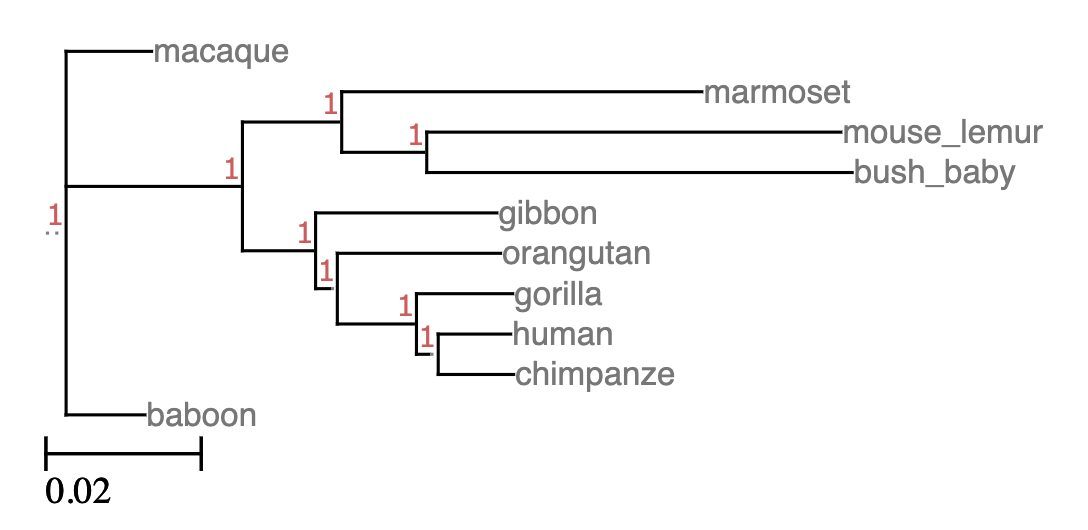
\includegraphics[width=\textwidth,height=8cm]{inferred_tree.png}
  \caption{Inferred primate phylogeny from our procedure.}
\end{figure}
\begin{figure}[H]
  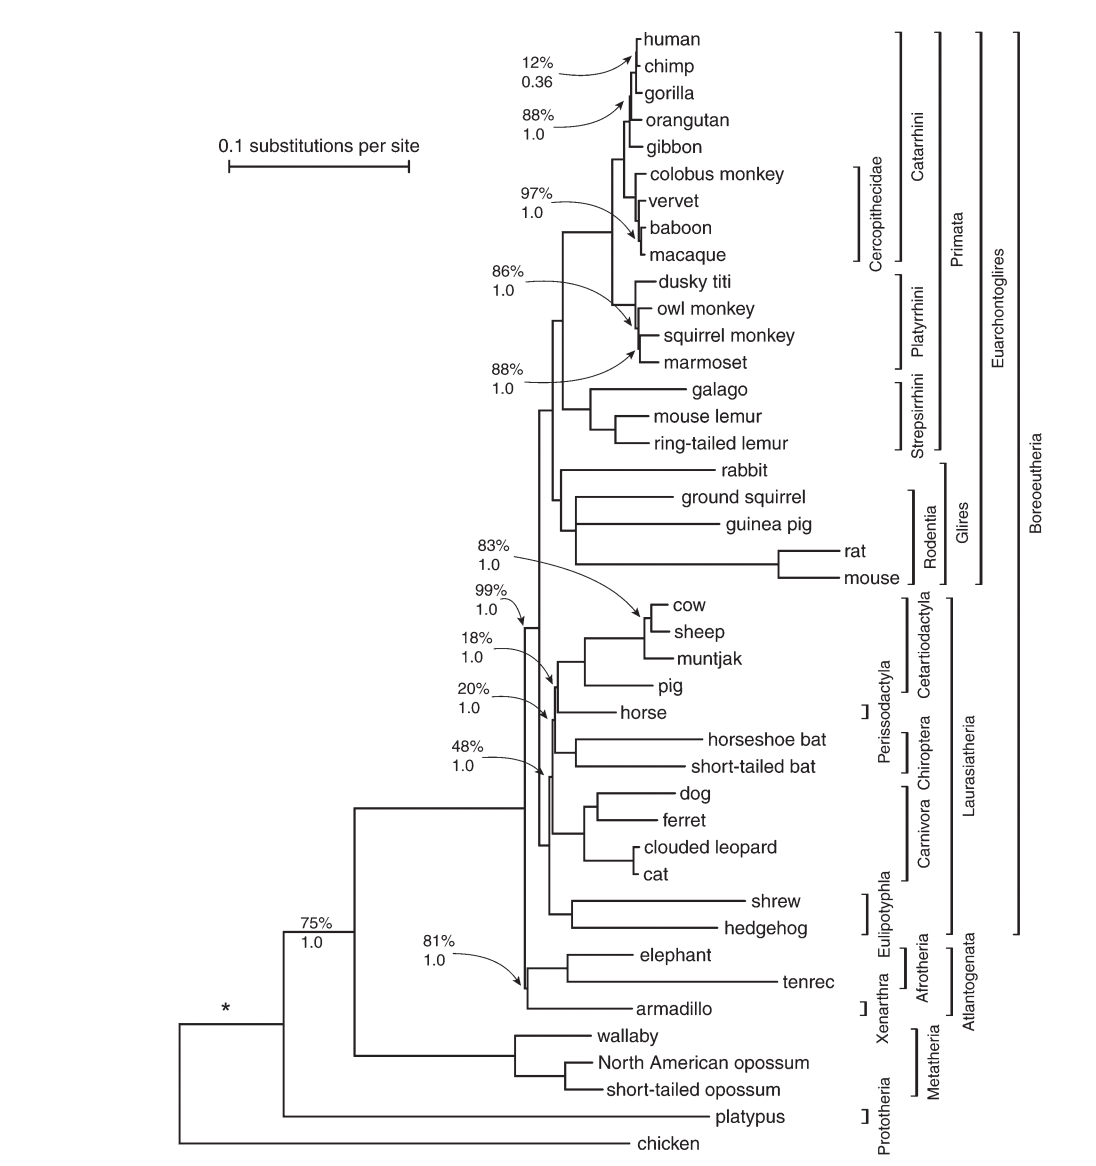
\includegraphics[width=\textwidth,height=16cm]{empirical_tree.png}
  \caption{Empirical primate phylogeny from Prasad et al. (2008).}
\end{figure}
\vspace{6cm}
% \color{black}
% \noindent\rule[0.25\baselineskip]{\textwidth}{1pt}
% Bibliography
% \small
%\bibliographystyle{unsrt}
\begin{thebibliography}{10}

\bibitem{1}
Baum, D. A., & Smith, S. D. (2013). Tree Thinking: An Introduction to Phylogenetic Biology. Greenwood Village, CO: Roberts and Company.
\bibitem{2}
Felsenstein J (2004). Inferring Phylogenies. Sunderland, Massachusetts: Sinauer Associates. ISBN 978-0-87893-177-4.

\bibitem{3}
Sankoff D, Morel C, Cedergren RJ (October 1973). "Evolution of 5S RNA and the non-randomness of base replacement". Nature. 245 (147): 232–4. doi:10.1038/newbio245232a0. PMID 4201431

\bibitem{4}
Wheeler WC, Gladstein DS (1994). "MALIGN: a multiple nucleic acid sequence alignment program". Journal of Heredity. 85 (5): 417–418. doi:10.1093/oxfordjournals.jhered.a111492.

\bibitem{5}
Cruaud, A. et al (2014). Empirical assessment of RAD sequencing for interspecific phylogeny. Mol. Biol. Evol. 31, 1272–1274.

\bibitem{6}
Andrews KR, Good JM, Miller MR, Luikart G, Hohenlohe PA (2016) Harnessing the power of
RADseq for ecological and evolutionary genomics. Nature Reviews Genetics, 17, 81–92. 

\bibitem{7}
Chong Z, Ruan J, Wu C-I (2012) Rainbow: an integrated tool for efficient clustering and
assembling RAD-seq reads. Bioinformatics, 28, 2732–2737. 

\bibitem{8}
Fan H, Ives AR, Surget-Groba Y, Cannon CH (2015) An assembly and alignment-free method of
phylogeny reconstruction from next-generation sequencing data. BMC Genomics, 16(1), 349.

\bibitem{9}
Stuart GW, Moffett K, Leader JJ. A Comprehensive Vertebrate Phylogeny Using Vector Representations of Protein Sequences from Whole Genomes. Mol Biol Evol. 2002;19:554–62.

\bibitem{10}
Prasad AB, Allard MW, NISC Comparative Sequencing Program, Green ED. Confirming the Phylogeny of Mammals by Use of Large Comparative Sequence Data Sets. Mol Biol Evol. 2008;25:1795–808.
\end{thebibliography}


\end{document}
